\subsection{ทดสอบประสิทธิภาพการทำงานของโมเดลปัญญาประดิษฐ์สำหรับการระบุตัวตนของบุคคล}
\label{sec:reid_ex}
ความแม่นยำของโมเดลปัญญาประดิษฐ์จากแหล่งที่มีมามีค่าดังตารางด้านล่างดังนี้
\begin{table}[!ht]
    \centering
    \begin{tabular}{|c|c|}
            \hline
            {โมเดลปัญญาประดิษฐ์}&{rank1/mAP โดยใช้วิธีการทดสอบด้วย Global+DMLI}				\\
            \hline
            ResNet50 Market1501	 			& 91.0/77.6								\\
            ResNet50 DukeMTMCReID			& 80.7/68.0								\\
            ResNet50 CUHK03				& 60.9/59.7								\\
            ResNet50 MSMT17				& 66.3/40.6								\\
        \hline
    \end{tabular}
    \caption{ผลการทดสอบความแม่นยำของโมเดลปัญญาประดิษฐ์}
    \label{tab: Accuracy of model ReID}
\end{table}
\\
ต่อมานำโมเดลปัญญาประดิษฐ์แต่ละอันมาทดสอบกับตัวอย่างภาพชุดข้อมูลที่ทางคณะผู้วิจัยได้สร้างขึ้น โดยภาพชุดข้อมูลที่นำมาใช้จะผ่านการตรวจหาบุคคลภายในภาพด้วยโมเดลปัญญาประดิษฐ์ YOLO-v3 spp และจะเป็นการทดลองในกรณีที่บุคคลในภาพนั้นเป็นบุคคลเดียวกัน
\begin{figure}[!ht]
    \centering
    \begin{subfigure}[b]{0.2\textwidth}
        \centering
        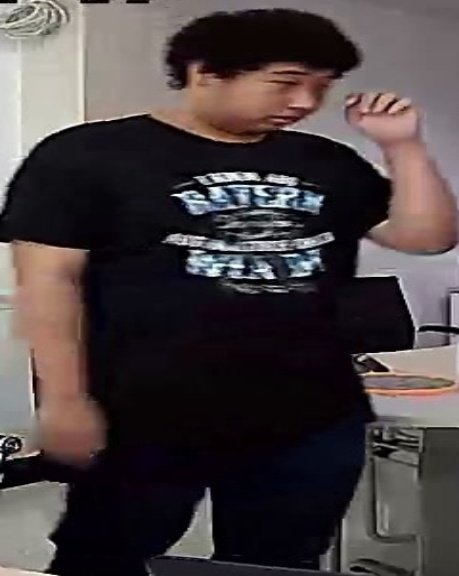
\includegraphics[width=\textwidth]{chapter4/images/o_0.jpg}
        \label{fig:ex_1}
    \end{subfigure}
    \begin{subfigure}[b]{0.2\textwidth}
        \centering
        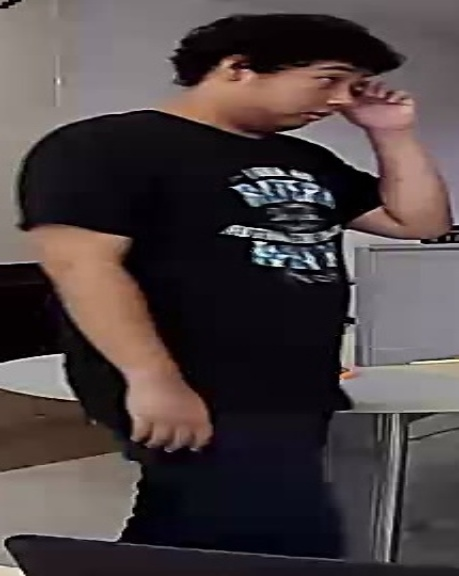
\includegraphics[width=\textwidth]{chapter4/images/o_1.jpg}
        \label{fig:ex_2}
    \end{subfigure}
    \caption{ภาพตัวอย่างชุดข้อมูลสำหรับการทดลองครั้งที่ 1}
    \label{fig: ภาพตัวอย่างชุดข้อมูลสำหรับการทดลอง 1}
\end{figure}

\begin{table}[!ht]
    \centering
    \begin{tabular}{|c|c|}
        \hline
        {โมเดลปัญญาประดิษฐ์}&{ค่าสำหรับการระบุตัวตนบุคคล (Original distance)}							\\
        \hline
        ResNet50 Market1501	 			& 0.4308								\\
        ResNet50 DukeMTMCReID			& 0.4827								\\
        ResNet50 CUHK03				& 0.4914								\\
        ResNet50 MSMT17				& 0.4668								\\
        \hline
    \end{tabular}
    \caption{ผลการทดสอบความแม่นยำสำหรับการระบุตัวตนบุคคลของโมเดลปัญญาประดิษฐ์ครั้งที่ 1}
    \label{tab: Original distant of image 1}
\end{table}
\clearpage
\begin{figure}[!ht]
    \centering
    \begin{subfigure}[b]{0.2\textwidth}
        \centering
        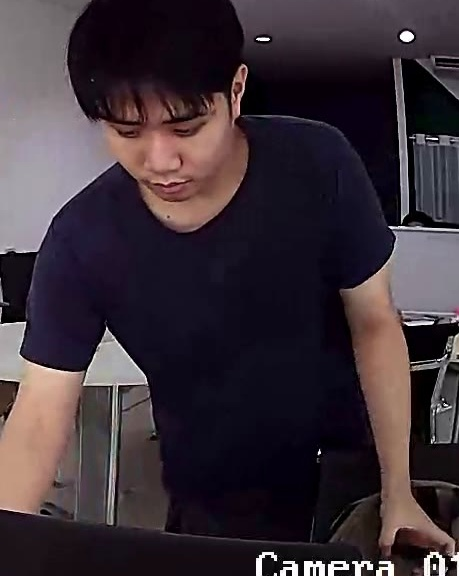
\includegraphics[width=\textwidth]{chapter4/images/first_0.jpg}
        \label{fig:ex_3}
    \end{subfigure}
    \begin{subfigure}[b]{0.2\textwidth}
        \centering
        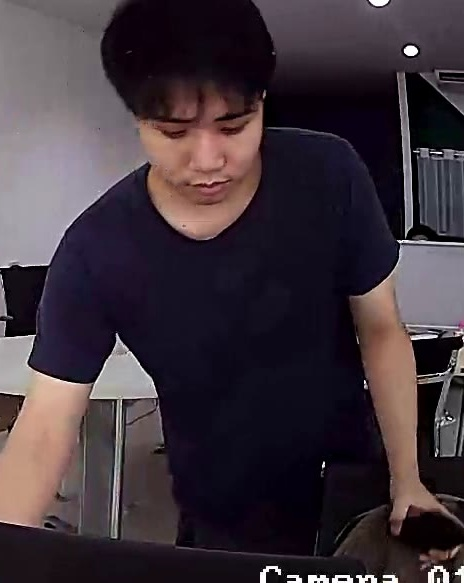
\includegraphics[width=\textwidth]{chapter4/images/first_1.jpg}
        \label{fig:ex_4}
    \end{subfigure}
    \caption{ภาพตัวอย่างชุดข้อมูลสำหรับการทดลองครั้งที่ 2}
    \label{fig: ภาพตัวอย่างชุดข้อมูลสำหรับการทดลอง 2}
\end{figure}
\begin{table}[!ht]
    \centering
    \begin{tabular}{|c|c|}
            \hline
            {โมเดลปัญญาประดิษฐ์}&{ค่าสำหรับการระบุตัวตนบุคคล (Original distance)}							\\
            \hline
            ResNet50 Market1501	 			& 0.3035								\\
            ResNet50 DukeMTMCReID			& 0.3332								\\
            ResNet50 CUHK03				& 0.3042								\\
            ResNet50 MSMT17				& 0.3684								\\
        \hline
    \end{tabular}
    \caption{ผลการทดสอบความแม่นยำสำหรับการระบุตัวตนบุคคลของโมเดลปัญญาประดิษฐ์ครั้งที่ 2}
    \label{tab: Original distant of image 2}    
\end{table}

\begin{figure}[!ht]
    \centering
    \begin{subfigure}[b]{0.2\textwidth}
        \centering
        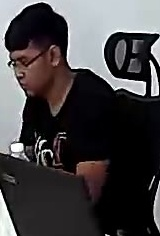
\includegraphics[width=\textwidth]{chapter4/images/fei_0.jpg}
        \label{fig:ex_5}
    \end{subfigure}
    \begin{subfigure}[b]{0.2\textwidth}
        \centering
        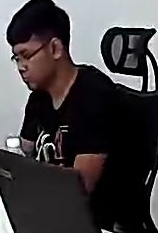
\includegraphics[width=\textwidth]{chapter4/images/fei_1.jpg}
        \label{fig:ex_6}
    \end{subfigure}
    \caption{ภาพตัวอย่างชุดข้อมูลสำหรับการทดลองครั้งที่ 3}
    \label{fig: ภาพตัวอย่างชุดข้อมูลสำหรับการทดลอง 3}
\end{figure}
\begin{table}[!ht]
    \centering
    \begin{tabular}{|c|c|}
		\hline
		{โมเดลปัญญาประดิษฐ์}&{ค่าสำหรับการระบุตัวตนบุคคล (Original distance)}							\\
		\hline
		ResNet50 Market1501	 			& 0.3308								\\
		ResNet50 DukeMTMCReID			& 0.3296								\\
		ResNet50 CUHK03				& 0.3134								\\
		ResNet50 MSMT17				& 0.3968								\\
	\hline
    \end{tabular}
    \caption{ผลการทดสอบความแม่นยำสำหรับการระบุตัวตนบุคคลของโมเดลปัญญาประดิษฐ์ครั้งที่ 3}
    \label{tab: Original distant of image 3}
\end{table}
\clearpage
ต่อมาจะเป็นการทดลองในกรณีที่บุคคลในภาพไม่เป็นบุคคลเดียวกัน
\begin{figure}[!ht]
    \centering
    \begin{subfigure}[b]{0.1\textwidth}
        \centering
        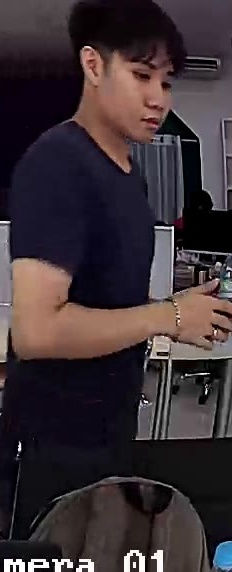
\includegraphics[width=\textwidth]{chapter4/images/first_3.jpg}
        \label{fig:ex_5}
    \end{subfigure}
    \begin{subfigure}[b]{0.1\textwidth}
        \centering
        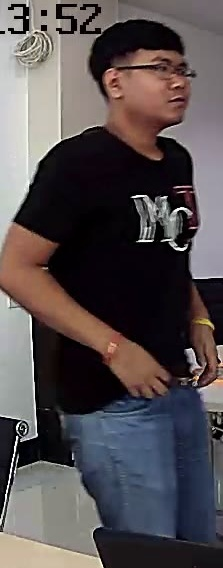
\includegraphics[width=\textwidth]{chapter4/images/fei_3.jpg}
        \label{fig:ex_6}
    \end{subfigure}
    \caption{ภาพตัวอย่างชุดข้อมูลสำหรับการทดลองครั้งที่ 4}
    \label{fig: ภาพตัวอย่างชุดข้อมูลสำหรับการทดลอง 4}
\end{figure}
\begin{table}[!ht]
    \centering
    \begin{tabular}{|c|c|}
		\hline
		{โมเดลปัญญาประดิษฐ์}&{ค่าสำหรับการระบุตัวตนบุคคล (Original distance)}							\\
		\hline
		ResNet50 Market1501	 			& 0.7285								\\
		ResNet50 DukeMTMCReID			& 0.6882								\\
		ResNet50 CUHK03				& 0.6727								\\
		ResNet50 MSMT17				& 0.7408								\\
	\hline
    \end{tabular}
    \caption{ผลการทดสอบความแม่นยำสำหรับการระบุตัวตนบุคคลของโมเดลปัญญาประดิษฐ์ครั้งที่ 4}
    \label{tab: Original distant of image 4}
\end{table}
\begin{figure}[!ht]
    \centering
    \begin{subfigure}[b]{0.1\textwidth}
        \centering
        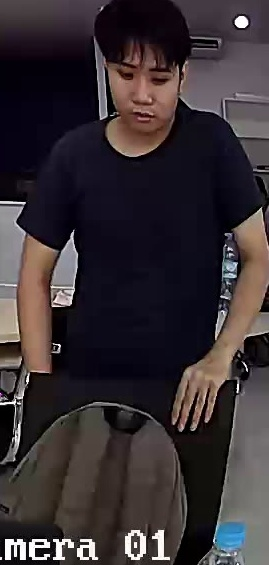
\includegraphics[width=\textwidth]{chapter4/images/first_4.jpg}
        \label{fig:ex_5}
    \end{subfigure}
    \begin{subfigure}[b]{0.1\textwidth}
        \centering
        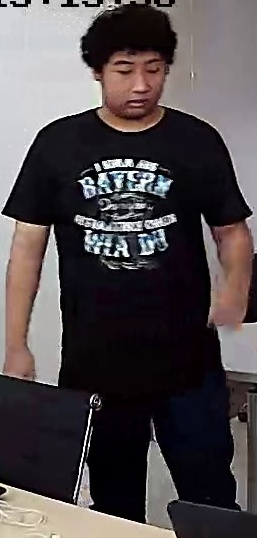
\includegraphics[width=\textwidth]{chapter4/images/o_3.jpg}
        \label{fig:ex_6}
    \end{subfigure}
    \caption{ภาพตัวอย่างชุดข้อมูลสำหรับการทดลองครั้งที่ 5}
    \label{fig: ภาพตัวอย่างชุดข้อมูลสำหรับการทดลอง 5}
\end{figure}
\begin{table}[!ht]
    \centering
    \begin{tabular}{|c|c|}
		\hline
		{โมเดลปัญญาประดิษฐ์}&{ค่าสำหรับการระบุตัวตนบุคคล (Original distance)}							\\
		\hline
		ResNet50 Market1501	 			& 0.6098								\\
		ResNet50 DukeMTMCReID			& 0.6522								\\
		ResNet50 CUHK03				& 0.6275								\\
		ResNet50 MSMT17				& 0.6155								\\
	\hline
    \end{tabular}
    \caption{ผลการทดสอบความแม่นยำสำหรับการระบุตัวตนบุคคลของโมเดลปัญญาประดิษฐ์ครั้งที่ 5}
    \label{tab: Original distant of image 5}
\end{table}
\clearpage
\begin{figure}[!ht]
    \centering
    \begin{subfigure}[b]{0.2\textwidth}
        \centering
        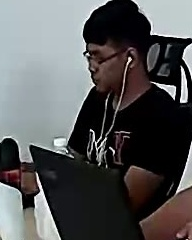
\includegraphics[width=\textwidth]{chapter4/images/fei_4.jpg}
        \label{fig:ex_5}
    \end{subfigure}
    \begin{subfigure}[b]{0.2\textwidth}
        \centering
        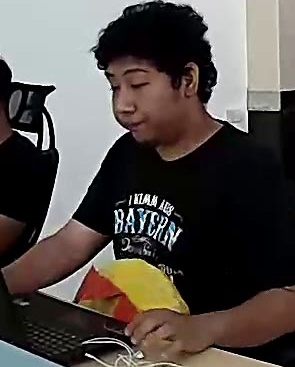
\includegraphics[width=\textwidth]{chapter4/images/o_4.jpg}
        \label{fig:ex_6}
    \end{subfigure}
    \caption{ภาพตัวอย่างชุดข้อมูลสำหรับการทดลองครั้งที่ 6}
    \label{fig: ภาพตัวอย่างชุดข้อมูลสำหรับการทดลอง 6}
\end{figure}
\begin{table}[!ht]
    \centering
    \begin{tabular}{|c|c|}
		\hline
		{โมเดลปัญญาประดิษฐ์}&{ค่าสำหรับการระบุตัวตนบุคคล (Original distance)}							\\
		\hline
		ResNet50 Market1501	 			& 0.6159								\\
		ResNet50 DukeMTMCReID			& 0.5352								\\
		ResNet50 CUHK03				& 0.5888								\\
		ResNet50 MSMT17				& 0.6119								\\
	\hline
    \end{tabular}
    \caption{ผลการทดสอบความแม่นยำสำหรับการระบุตัวตนบุคคลของโมเดลปัญญาประดิษฐ์ครั้งที่ 6}
    \label{tab: Original distant of image 6}
\end{table}

ค่าความแม่นยำในการระบุตัวตนบุคคลนั้นค่ายิ่งเข้าใกล้ 0 แสดงบุคคลใน 2 เฟรมนั้นเป็นบุคคลเดียวกัน จากการทดลองครั้งที่ 1 จะเป็นเฟรมที่ไม่ต่อเนื่องกัน การทดลองครั้งที่ 2 และ 3 นั้นจะเป็นเฟรมที่ต่อเนื่องกันมากขึ้นตามลำดับ และการทดลองที่ 4 5 และ 6 นั้นจะนำภาพที่แต่ละบุคคลที่ท่าทางใกล้เคียงกันมาใช้ ซึ่งจะแสดงให้เห็นว่าโมเดลปัญญาประดิษฐ์ที่สามารถให้ผลลัพธ์ที่มีประสิทธิภาพต่อเนื่องมากที่สุดคือ ResNet50 Market1501
